\documentclass[11pt, a4paper]{article}\usepackage[]{graphicx}\usepackage[]{xcolor}
% maxwidth is the original width if it is less than linewidth
% otherwise use linewidth (to make sure the graphics do not exceed the margin)
\makeatletter
\def\maxwidth{ %
  \ifdim\Gin@nat@width>\linewidth
    \linewidth
  \else
    \Gin@nat@width
  \fi
}
\makeatother

\definecolor{fgcolor}{rgb}{0.345, 0.345, 0.345}
\newcommand{\hlnum}[1]{\textcolor[rgb]{0.686,0.059,0.569}{#1}}%
\newcommand{\hlstr}[1]{\textcolor[rgb]{0.192,0.494,0.8}{#1}}%
\newcommand{\hlcom}[1]{\textcolor[rgb]{0.678,0.584,0.686}{\textit{#1}}}%
\newcommand{\hlopt}[1]{\textcolor[rgb]{0,0,0}{#1}}%
\newcommand{\hlstd}[1]{\textcolor[rgb]{0.345,0.345,0.345}{#1}}%
\newcommand{\hlkwa}[1]{\textcolor[rgb]{0.161,0.373,0.58}{\textbf{#1}}}%
\newcommand{\hlkwb}[1]{\textcolor[rgb]{0.69,0.353,0.396}{#1}}%
\newcommand{\hlkwc}[1]{\textcolor[rgb]{0.333,0.667,0.333}{#1}}%
\newcommand{\hlkwd}[1]{\textcolor[rgb]{0.737,0.353,0.396}{\textbf{#1}}}%
\let\hlipl\hlkwb

\usepackage{framed}
\makeatletter
\newenvironment{kframe}{%
 \def\at@end@of@kframe{}%
 \ifinner\ifhmode%
  \def\at@end@of@kframe{\end{minipage}}%
  \begin{minipage}{\columnwidth}%
 \fi\fi%
 \def\FrameCommand##1{\hskip\@totalleftmargin \hskip-\fboxsep
 \colorbox{shadecolor}{##1}\hskip-\fboxsep
     % There is no \\@totalrightmargin, so:
     \hskip-\linewidth \hskip-\@totalleftmargin \hskip\columnwidth}%
 \MakeFramed {\advance\hsize-\width
   \@totalleftmargin\z@ \linewidth\hsize
   \@setminipage}}%
 {\par\unskip\endMakeFramed%
 \at@end@of@kframe}
\makeatother

\definecolor{shadecolor}{rgb}{.97, .97, .97}
\definecolor{messagecolor}{rgb}{0, 0, 0}
\definecolor{warningcolor}{rgb}{1, 0, 1}
\definecolor{errorcolor}{rgb}{1, 0, 0}
\newenvironment{knitrout}{}{} % an empty environment to be redefined in TeX

\usepackage{alltt}

\usepackage[top=1 in, bottom = 1 in, left = 1 in, right = 1 in ]{geometry}

\usepackage{amsmath, amssymb, amsfonts}
\usepackage{enumerate}
\usepackage{float}

\title{One Way ANOVA - An Agricultural Example}
\author{Ananda Biswas}
\date{}
\IfFileExists{upquote.sty}{\usepackage{upquote}}{}
\begin{document}

\maketitle

Suppose we have 8 plots and 3 varieties of a crop. We want to study the yield of the different varieties of the crop.


\begin{table}[H]

\begin{center}

\begin{tabular}{cccc}


\includegraphics[scale = 0.5]{plot 1} & 
\includegraphics[scale = 0.52]{plot 2} & 
\includegraphics[scale = 0.5]{plot 3} & 
\includegraphics[scale = 0.5]{plot 4}\\


\includegraphics[scale = 0.51]{plot 5} & 
\includegraphics[scale = 0.5]{plot 6} & 
\includegraphics[scale = 0.5]{plot 7} & 
\includegraphics[scale = 0.5]{plot 8}\\
\end{tabular}

\end{center}

\end{table}


First we randomly select 3 plots for variety \textbf{1}, then another 3 plots for variety \textbf{2} and the rest 2 plots are used for variety \textbf{3}.

\begin{figure}[H]
  \centering
  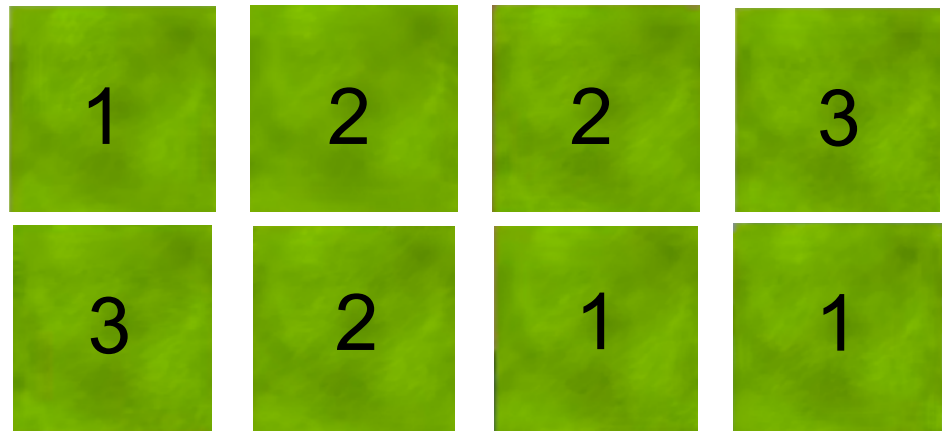
\includegraphics[scale = 0.45]{allocation} \\
\end{figure}


Here our blackbox diagram is
\begin{figure}[H]
  \centering
  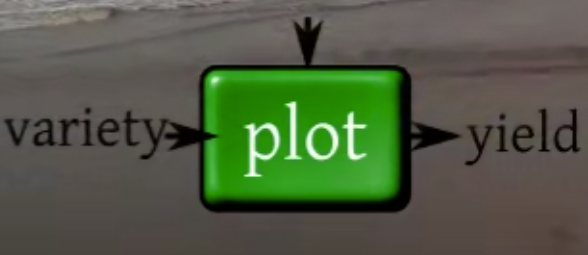
\includegraphics[scale = 0.5]{blackbox} \\
\end{figure}


\newpage


Our data set is

\begin{figure}[H]
  \centering
  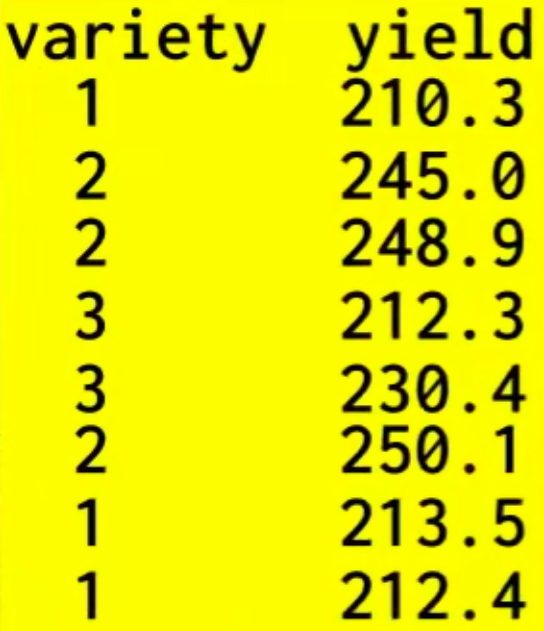
\includegraphics[scale = 0.5]{dataset} \\
\end{figure}


We can have a linear model as follows :

$$y_{ij} = \alpha_i + \epsilon_{ij}$$

where $y_{ij}$ is the observed yield in the $jth$ plot of the $ith$ variety of crop ; \\

$\alpha_i$ is the true yield of the $ith$ variety of crop; \\

$\epsilon_{ij}$ is the random error in the $jth$ plot of the $ith$ variety of crop. \\

Here, $i = 1, 2, 3$. For $i = 1, 2$, $j = 1, 2, 3$ and for $i = 3$, $j = 1, 2$. \\

$\bullet$ We may be interested in seeing which variety of the crop gives more yield. Then we can come up with another linear model :

$$y_{ij} = \mu + \alpha_i + \epsilon_{ij}$$

where $\mu$ is on an average, the true yield of the crop for all varieties; \\

$\alpha_i$ is the additional yield of the $ith$ variety of the crop. \\

See that $\mu$ is unidentifiable from the above model. \\

We shall put a restriction on $\alpha_i$s that $\sum\limits_{i = 1}^3 \alpha_i = 0$. This also boosts the interpretation of the model - $\mu$ is the average yield of the crop; $\alpha_i$ is additional yield of $i$th variety. So when we average the true yields of all the varieties, we get $\mu$. \Big[$\dfrac{1}{3}\sum\limits_{i=1}^3 (\mu + \alpha_i) = \mu \Big]$ \\

$\bullet$ Suppose variety \textbf{1} of the crop is widely used, 2 new varieties of the crop has been discovered and we want to study their effectiveness. \\

In such a scenario, yet another linear model can be :

$$y_{ij} = \mu + \alpha_i + \epsilon_{ij}$$

where $\mu$ is the benchmark yield of the crop when variety \textbf{1} is used; \\

$\alpha_1 = 0$, and $\alpha_2$, $\alpha_3$ are additional yields of the variety \textbf{2} and variety \textbf{3} respectively.


\begin{knitrout}
\definecolor{shadecolor}{rgb}{0.969, 0.969, 0.969}\color{fgcolor}\begin{kframe}
\begin{alltt}
\hlkwd{getwd}\hlstd{()}
\end{alltt}
\begin{verbatim}
## [1] "D:/Programming Languages/R/Linear Statistical Models - Arnab Chakraborty/004"
\end{verbatim}
\end{kframe}
\end{knitrout}

\begin{knitrout}
\definecolor{shadecolor}{rgb}{0.969, 0.969, 0.969}\color{fgcolor}\begin{kframe}
\begin{alltt}
\hlstd{agri} \hlkwb{=} \hlkwd{read.csv}\hlstd{(}\hlstr{'variety_and_yield_dataset.csv'}\hlstd{)}

\hlstd{agri}
\end{alltt}
\begin{verbatim}
##   variety yield
## 1       1 210.3
## 2       2 245.0
## 3       2 248.9
## 4       3 212.3
## 5       3 230.4
## 6       2 250.1
## 7       1 213.5
## 8       1 212.4
\end{verbatim}
\begin{alltt}
\hlkwd{dim}\hlstd{(agri)}
\end{alltt}
\begin{verbatim}
## [1] 8 2
\end{verbatim}
\begin{alltt}
\hlkwd{names}\hlstd{(agri)}
\end{alltt}
\begin{verbatim}
## [1] "variety" "yield"
\end{verbatim}
\end{kframe}
\end{knitrout}

The variable \textit{variety} is a factor.

\begin{knitrout}
\definecolor{shadecolor}{rgb}{0.969, 0.969, 0.969}\color{fgcolor}\begin{kframe}
\begin{alltt}
\hlstd{agri}\hlopt{$}\hlstd{variety} \hlkwb{=} \hlkwd{factor}\hlstd{(agri}\hlopt{$}\hlstd{variety)}
\end{alltt}
\end{kframe}
\end{knitrout}

\begin{knitrout}
\definecolor{shadecolor}{rgb}{0.969, 0.969, 0.969}\color{fgcolor}\begin{kframe}
\begin{alltt}
\hlkwd{library}\hlstd{(tidyverse)}
\end{alltt}


{\ttfamily\noindent\color{warningcolor}{\#\# Warning: package 'tidyverse' was built under R version 4.2.3}}

{\ttfamily\noindent\color{warningcolor}{\#\# Warning: package 'ggplot2' was built under R version 4.2.2}}

{\ttfamily\noindent\color{warningcolor}{\#\# Warning: package 'tibble' was built under R version 4.2.3}}

{\ttfamily\noindent\color{warningcolor}{\#\# Warning: package 'tidyr' was built under R version 4.2.3}}

{\ttfamily\noindent\color{warningcolor}{\#\# Warning: package 'readr' was built under R version 4.2.2}}

{\ttfamily\noindent\color{warningcolor}{\#\# Warning: package 'purrr' was built under R version 4.2.3}}

{\ttfamily\noindent\color{warningcolor}{\#\# Warning: package 'dplyr' was built under R version 4.2.3}}

{\ttfamily\noindent\color{warningcolor}{\#\# Warning: package 'stringr' was built under R version 4.2.3}}

{\ttfamily\noindent\color{warningcolor}{\#\# Warning: package 'forcats' was built under R version 4.2.2}}

{\ttfamily\noindent\color{warningcolor}{\#\# Warning: package 'lubridate' was built under R version 4.2.2}}

{\ttfamily\noindent\itshape\color{messagecolor}{\#\# -- Attaching core tidyverse packages ------------------------ tidyverse 2.0.0 --\\\#\# v dplyr \ \ \ \ 1.1.3 \ \ \ \ v readr \ \ \ \ 2.1.4\\\#\# v forcats \ \ 1.0.0 \ \ \ \ v stringr \ \ 1.5.0\\\#\# v ggplot2 \ \ 3.4.1 \ \ \ \ v tibble \ \ \ 3.2.1\\\#\# v lubridate 1.9.2 \ \ \ \ v tidyr \ \ \ \ 1.3.0\\\#\# v purrr \ \ \ \ 1.0.2 \ \ \ \ \\\#\# -- Conflicts ------------------------------------------ tidyverse\_conflicts() --\\\#\# x dplyr::filter() masks stats::filter()\\\#\# x dplyr::lag() \ \ \ masks stats::lag()\\\#\# i Use the conflicted package (<http://conflicted.r-lib.org/>) to force all conflicts to become errors}}\begin{alltt}
\hlstd{agri} \hlopt
  \hlkwd{ggplot}\hlstd{(}\hlkwd{aes}\hlstd{(}\hlkwc{x} \hlstd{= variety,} \hlkwc{y} \hlstd{= yield))} \hlopt{+}
  \hlkwd{stat_boxplot}\hlstd{(}\hlkwc{geom} \hlstd{=} \hlstr{"errorbar"}\hlstd{,} \hlkwc{linewidth} \hlstd{=} \hlnum{1}\hlstd{)} \hlopt{+}
  \hlkwd{geom_boxplot}\hlstd{(}\hlkwc{fill} \hlstd{=} \hlstr{"#31F30A"}\hlstd{,} \hlkwc{color} \hlstd{=} \hlstr{"black"}\hlstd{)} \hlopt{+}
  \hlkwd{labs}\hlstd{(}\hlkwc{x} \hlstd{=} \hlstr{"Variety"}\hlstd{,} \hlkwc{y} \hlstd{=} \hlstr{"Yield"}\hlstd{,} \hlkwc{title} \hlstd{=} \hlstr{"Boxplot of Yields of Different Varieties"}\hlstd{)}
\end{alltt}
\end{kframe}
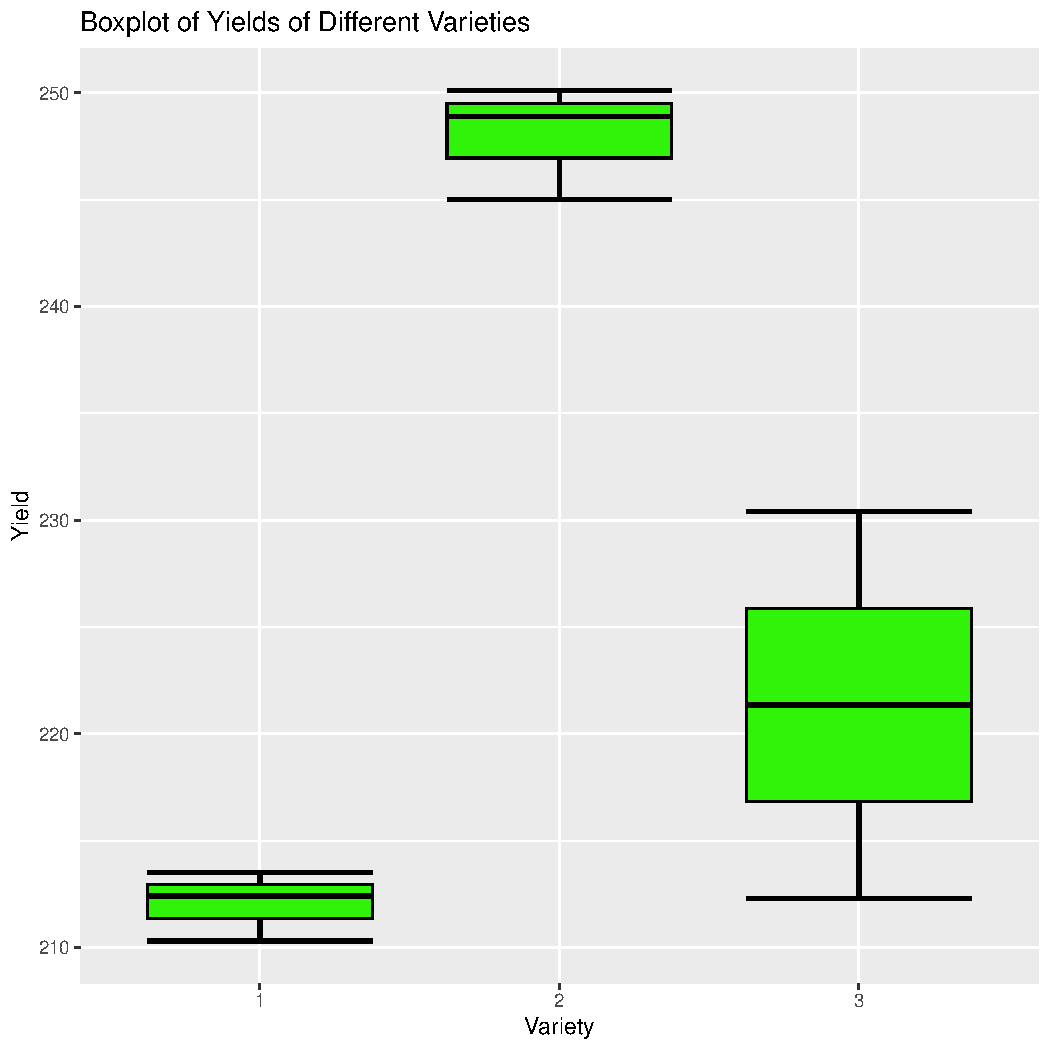
\includegraphics[width=\maxwidth]{figure/unnamed-chunk-4-1} 
\end{knitrout}

We shall fit the model :

$$y_{ij} = \mu + \alpha_i + \epsilon_{ij}$$

where $\mu$ is on an average, the true yield of the crop for all varieties; \\

$\alpha_i$ is the additional yield of the $ith$ variety of the crop.

\begin{knitrout}
\definecolor{shadecolor}{rgb}{0.969, 0.969, 0.969}\color{fgcolor}\begin{kframe}
\begin{alltt}
\hlstd{fit1} \hlkwb{=} \hlkwd{lm}\hlstd{(yield} \hlopt{~} \hlstd{variety, agri)}
\end{alltt}
\end{kframe}
\end{knitrout}

\begin{knitrout}
\definecolor{shadecolor}{rgb}{0.969, 0.969, 0.969}\color{fgcolor}\begin{kframe}
\begin{alltt}
\hlstd{fit1}
\end{alltt}
\begin{verbatim}
## 
## Call:
## lm(formula = yield ~ variety, data = agri)
## 
## Coefficients:
## (Intercept)     variety2     variety3  
##     212.067       35.933        9.283
\end{verbatim}
\end{kframe}
\end{knitrout}

Surprisingly, we do not get any estimate for \textbf{variety1}. Let's see the model matrix.
\begin{knitrout}
\definecolor{shadecolor}{rgb}{0.969, 0.969, 0.969}\color{fgcolor}\begin{kframe}
\begin{alltt}
\hlkwd{model.matrix}\hlstd{(fit1)}
\end{alltt}
\begin{verbatim}
##   (Intercept) variety2 variety3
## 1           1        0        0
## 2           1        1        0
## 3           1        1        0
## 4           1        0        1
## 5           1        0        1
## 6           1        1        0
## 7           1        0        0
## 8           1        0        0
## attr(,"assign")
## [1] 0 1 1
## attr(,"contrasts")
## attr(,"contrasts")$variety
## [1] "contr.treatment"
\end{verbatim}
\end{kframe}
\end{knitrout}

R never constructs a model matrix that is not full column rank. If the design matrix does not become full column rank, R will throw away columns to make it full column rank. \\

Here $\alpha_1$ is forced to be $0$. \\

Let us fit the linaer model :

$$y_{ij} = \alpha_i + \epsilon_{ij}$$

where $y_{ij}$ is the observed yield in the $jth$ plot of the $ith$ variety of crop ; \\

$\alpha_i$ is the true yield of the $ith$ variety of crop.

\begin{knitrout}
\definecolor{shadecolor}{rgb}{0.969, 0.969, 0.969}\color{fgcolor}\begin{kframe}
\begin{alltt}
\hlstd{fit2} \hlkwb{=} \hlkwd{lm}\hlstd{(yield} \hlopt{~} \hlstd{variety} \hlopt{-} \hlnum{1}\hlstd{, agri)}
\end{alltt}
\end{kframe}
\end{knitrout}

\begin{knitrout}
\definecolor{shadecolor}{rgb}{0.969, 0.969, 0.969}\color{fgcolor}\begin{kframe}
\begin{alltt}
\hlstd{fit2}
\end{alltt}
\begin{verbatim}
## 
## Call:
## lm(formula = yield ~ variety - 1, data = agri)
## 
## Coefficients:
## variety1  variety2  variety3  
##    212.1     248.0     221.3
\end{verbatim}
\end{kframe}
\end{knitrout}

\begin{knitrout}
\definecolor{shadecolor}{rgb}{0.969, 0.969, 0.969}\color{fgcolor}\begin{kframe}
\begin{alltt}
\hlkwd{model.matrix}\hlstd{(fit2)}
\end{alltt}
\begin{verbatim}
##   variety1 variety2 variety3
## 1        1        0        0
## 2        0        1        0
## 3        0        1        0
## 4        0        0        1
## 5        0        0        1
## 6        0        1        0
## 7        1        0        0
## 8        1        0        0
## attr(,"assign")
## [1] 1 1 1
## attr(,"contrasts")
## attr(,"contrasts")$variety
## [1] "contr.treatment"
\end{verbatim}
\end{kframe}
\end{knitrout}

See that previously $\alpha_1$ was forced to $0$. We can interpret that variety \textbf{1} is the benchmark variety and the intercept is benchmark yield. 

\begin{knitrout}
\definecolor{shadecolor}{rgb}{0.969, 0.969, 0.969}\color{fgcolor}\begin{kframe}
\begin{alltt}
\hlstd{fit1}\hlopt{$}\hlstd{coefficients}
\end{alltt}
\begin{verbatim}
## (Intercept)    variety2    variety3 
##  212.066667   35.933333    9.283333
\end{verbatim}
\end{kframe}
\end{knitrout}

\begin{knitrout}
\definecolor{shadecolor}{rgb}{0.969, 0.969, 0.969}\color{fgcolor}\begin{kframe}
\begin{alltt}
\hlstd{fit2}\hlopt{$}\hlstd{coefficients}
\end{alltt}
\begin{verbatim}
## variety1 variety2 variety3 
## 212.0667 248.0000 221.3500
\end{verbatim}
\end{kframe}
\end{knitrout}

In \textbf{fit1}, R has reported the benchmark yield and the \textit{additional yields from variety \textbf{1}} of variety \textbf{2} and \textbf{3}. \\

In \textbf{fit2}, R has reported the estimated yields of all the varieties. \\

We can easily observe that, the two reports are equivalent. If we add the intercept(the benchmark yield) and add additional yield of variety2, variety3 in \textbf{fit1}, we can get the estimated yield of variety \textbf{2} and \textbf{3} as given by fit2 respectively. \\

We can also estimate $\sigma^2$.

\begin{knitrout}
\definecolor{shadecolor}{rgb}{0.969, 0.969, 0.969}\color{fgcolor}\begin{kframe}
\begin{alltt}
\hlkwd{summary}\hlstd{(fit1)}
\end{alltt}
\begin{verbatim}
## 
## Call:
## lm(formula = yield ~ variety, data = agri)
## 
## Residuals:
##       1       2       3       4       5       6       7       8 
## -1.7667 -3.0000  0.9000 -9.0500  9.0500  2.1000  1.4333  0.3333 
## 
## Coefficients:
##             Estimate Std. Error t value Pr(>|t|)    
## (Intercept)  212.067      3.496  60.663  2.3e-08 ***
## variety2      35.933      4.944   7.268 0.000771 ***
## variety3       9.283      5.527   1.680 0.153887    
## ---
## Signif. codes:  0 '***' 0.001 '**' 0.01 '*' 0.05 '.' 0.1 ' ' 1
## 
## Residual standard error: 6.055 on 5 degrees of freedom
## Multiple R-squared:  0.9179,	Adjusted R-squared:  0.8851 
## F-statistic: 27.96 on 2 and 5 DF,  p-value: 0.00193
\end{verbatim}
\end{kframe}
\end{knitrout}

The \textbf{Residual standard error} is the estimated $\sigma^2$.






\end{document}
